\documentclass[11pt,a4paper]{article}
\usepackage[utf8]{inputenc}
\usepackage[T1]{fontenc}
\usepackage{geometry}
\usepackage{xcolor}
\usepackage{tcolorbox}
\usepackage{enumitem}
\usepackage{hyperref}
\usepackage{booktabs}
\usepackage{longtable}
\usepackage{graphicx}
\usepackage{fancyhdr}
\usepackage{pgfplots}
\usepackage{tikz}
\usepackage[table]{xcolor}
\pgfplotsset{compat=1.18}

\definecolor{tablerowgray}{RGB}{245,245,245}

\geometry{margin=1in}
\setlength{\headheight}{14pt}

\definecolor{strengthgreen}{RGB}{46,125,50}
\definecolor{warningorange}{RGB}{245,124,0}
\definecolor{criticalred}{RGB}{198,40,40}
\definecolor{infocolor}{RGB}{33,33,33}

\pagestyle{fancy}
\fancyhf{}
\rhead{Architectural Validation Report}
\lhead{Library Management System}
\rfoot{Page \thepage}

\title{\textbf{Architectural Blueprint Validation Report}\\
\large Library Management System}
\author{Automated Traceability Analysis}
\date{\today}

\begin{document}

\maketitle

\begin{abstract}
This report validates the architectural blueprint of the Library Management System through automated traceability analysis. The assessment examines 3 requirements, 8 use cases, architectural components, and test coverage extracted via LLM-based document analysis. The report identifies critical gaps in test coverage, architectural clarity, and use case specification, providing actionable recommendations for improving system design quality.
\end{abstract}

\tableofcontents
\newpage

\section{Executive Summary}

\subsection{Assessment Overview}

This validation analyzes the architectural blueprint using automated traceability extraction from project documentation. The system demonstrates strong architectural layering with comprehensive DAO patterns but exhibits significant gaps in test coverage for use case workflows and vague component responsibilities requiring clarification.

\subsubsection{Coverage Metrics}

Table~\ref{tab:metrics-summary} provides a high-level summary of key project metrics, while Figures~\ref{fig:coverage-metrics} and~\ref{fig:test-distribution} visualize the coverage distribution and test composition.

\begin{table}[h]
\centering
\begin{tabular}{@{}lrrr@{}}
\toprule
\textbf{Metric Category} & \textbf{Total} & \textbf{Covered} & \textbf{Coverage} \\
\midrule
Requirements & 3 & 3 & 100\% \\
Use Cases & 8 & 2 & 25\% \\
Tests & 113 & 113 & 100\% \\
Architecture Layers & 6 & 6 & 100\% \\
Critical Risks & 3 & --- & 2 Critical, 1 High \\
\bottomrule
\end{tabular}
\caption{Project Metrics Summary}
\label{tab:metrics-summary}
\end{table}

Figure~\ref{fig:coverage-metrics} visualizes the overall coverage across requirements and use cases, while Figure~\ref{fig:test-distribution} shows the test composition by type.

\begin{figure}[h]
\centering
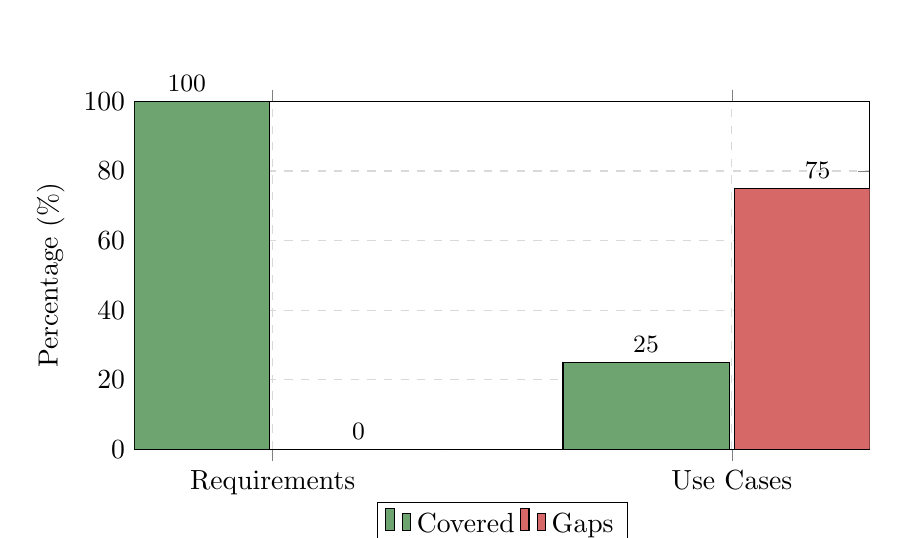
\begin{tikzpicture}
\begin{axis}[
    ybar,
    width=0.9\textwidth,
    height=6cm,
    ylabel={Percentage (\%)},
    symbolic x coords={Requirements, Use Cases},
    xtick=data,
    ymin=0, ymax=100,
    bar width=60pt,
    enlarge x limits=0.3,
    legend style={at={(0.5,-0.15)}, anchor=north, legend columns=-1},
    nodes near coords,
    nodes near coords style={font=\small},
    grid=major,
    grid style={dashed,gray!30}
]
\addplot[fill=strengthgreen!70] coordinates {(Requirements,100) (Use Cases,25)};
\addplot[fill=criticalred!70] coordinates {(Requirements,0) (Use Cases,75)};
\legend{Covered, Gaps}
\end{axis}
\end{tikzpicture}
\caption{Requirements and Use Case Coverage}
\label{fig:coverage-metrics}
\end{figure}

\begin{figure}[h]
\centering
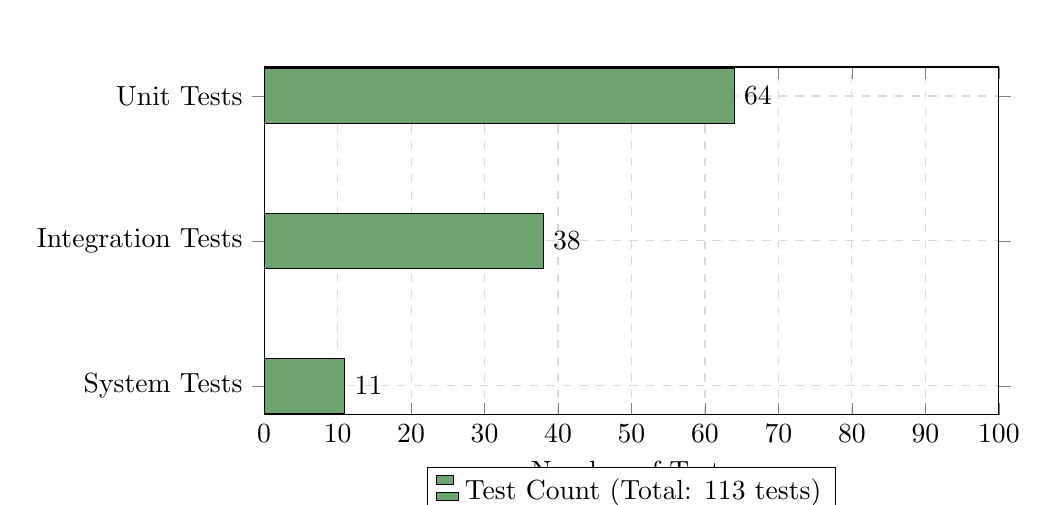
\begin{tikzpicture}
\begin{axis}[
    xbar,
    width=0.9\textwidth,
    height=6cm,
    xlabel={Number of Tests},
    symbolic y coords={System Tests, Integration Tests, Unit Tests},
    ytick=data,
    xmin=0, xmax=100,
    bar width=20pt,
    nodes near coords,
    nodes near coords align={horizontal},
    grid=major,
    grid style={dashed,gray!30},
    legend style={at={(0.5,-0.15)}, anchor=north, legend columns=-1}
]
\addplot[fill=strengthgreen!70] coordinates {(64,{Unit Tests}) (38,{Integration Tests}) (11,{System Tests})};
\legend{Test Count (Total: 113 tests)}
\end{axis}
\end{tikzpicture}
\caption{Test Distribution by Type (Total: 113 tests)}
\label{fig:test-distribution}
\end{figure}

\subsubsection{Risk Distribution}

Figure~\ref{fig:risk-distribution} presents the distribution of identified risks by severity level, highlighting the critical issues requiring immediate attention.

\begin{figure}[h]
\centering
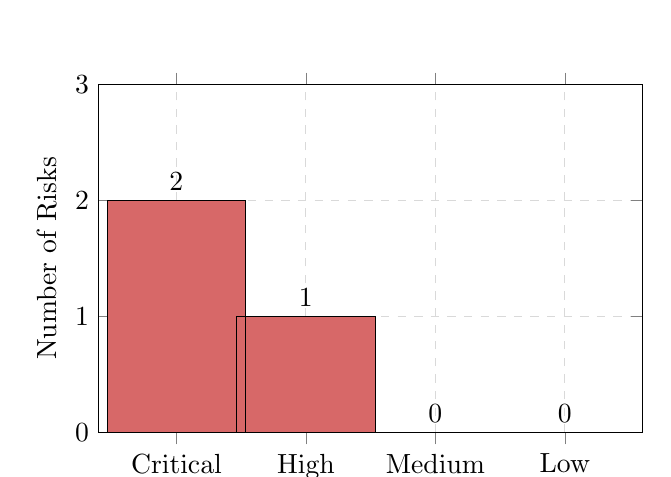
\begin{tikzpicture}
\begin{axis}[
    ybar,
    width=0.7\textwidth,
    height=6cm,
    ylabel={Number of Risks},
    symbolic x coords={Critical, High, Medium, Low},
    xtick=data,
    ymin=0, ymax=3,
    bar width=50pt,
    enlarge x limits=0.2,
    nodes near coords,
    nodes near coords style={font=\normalsize},
    grid=major,
    grid style={dashed,gray!30}
]
\addplot[fill=criticalred!70] coordinates {(Critical,2) (High,1) (Medium,0) (Low,0)};
\end{axis}
\end{tikzpicture}
\caption{Risk Distribution by Severity (Total: 3 risks)}
\label{fig:risk-distribution}
\end{figure}

\subsection{Critical Findings}

\begin{tcolorbox}[colback=criticalred!5,colframe=criticalred,title=\textbf{Critical Issues Requiring Immediate Attention}]
\begin{enumerate}
    \item \textbf{Severe Use Case Test Coverage Gap:} Six of eight use cases (75\%) lack corresponding test coverage, with four use cases having no tests whatsoever, creating validation blind spots in critical workflows.

    \item \textbf{Vague Component Responsibilities:} Multiple architectural components lack precise responsibility definitions, violating the Single Responsibility Principle and risking architectural erosion during maintenance.

    \item \textbf{Orphaned Use Cases:} Two use cases function as organizational containers with no defined flows, creating confusion in the use case model and providing no traceability value.
\end{enumerate}
\end{tcolorbox}

\begin{tcolorbox}[colback=strengthgreen!5,colframe=strengthgreen,title=\textbf{Architectural Strengths}]
\begin{itemize}[leftmargin=*]
    \item Complete requirement-to-architecture mapping with full coverage
    \item Well-defined layered architecture with proper separation of concerns
    \item Comprehensive DAO pattern implementation across all entity types
    \item Effective use of design patterns (Builder, DAO, Mapper) applied strategically
    \item Extensive unit test suite with 113 total tests providing strong code coverage
    \item Clear inheritance hierarchy for user role management
\end{itemize}
\end{tcolorbox}

\section{Project Inventory}

This section provides a complete inventory of all requirements, use cases, and tests identified in the system. All subsequent sections reference these items by their IDs.

\subsection{Requirements Inventory}

Table~\ref{tab:all-requirements} provides a comprehensive list of all 3 requirements identified in the system, categorized by functional area. The coverage status indicates whether each requirement is supported by the current architecture.

\rowcolors{2}{white}{tablerowgray}
\begin{longtable}{@{}p{0.12\textwidth}p{0.52\textwidth}p{0.15\textwidth}p{0.12\textwidth}@{}}
\caption{Complete Requirements List} \label{tab:all-requirements} \\
\toprule
\rowcolor{white}\textbf{ID} & \textbf{Requirement Description} & \textbf{Category} & \textbf{Status} \\
\midrule
\endfirsthead

\multicolumn{4}{c}%
{{\tablename\ \thetable{} -- continued from previous page}} \\
\toprule
\rowcolor{white}\textbf{ID} & \textbf{Requirement Description} & \textbf{Category} & \textbf{Status} \\
\midrule
\endhead

\midrule
\multicolumn{4}{r}{{Continued on next page}} \\
\endfoot

\bottomrule
\endlastfoot

\label{req:1}\hyperref[req:1]{REQ-1} & The system must allow users to borrow and return books, digital media, and periodicals & Functional & Covered \\
\label{req:2}\hyperref[req:2]{REQ-2} & The system must allow administrators to add, modify, and remove catalog items & Functional & Covered \\
\label{req:3}\hyperref[req:3]{REQ-3} & The system must handle any product within the library catalog as an element, regardless of its specific type & Goal/Background & Covered \\
\end{longtable}

\subsection{Use Cases Inventory}

Table~\ref{tab:all-usecases} provides a complete list of all 8 use cases defined in the system, along with their primary actors, descriptions, and test coverage status.

\rowcolors{2}{white}{tablerowgray}
\begin{longtable}{@{}p{0.10\textwidth}p{0.30\textwidth}p{0.13\textwidth}p{0.10\textwidth}p{0.22\textwidth}@{}}
\caption{Complete Use Cases List} \label{tab:all-usecases} \\
\toprule
\rowcolor{white}\textbf{ID} & \textbf{Use Case Name} & \textbf{Actor} & \textbf{Tests} & \textbf{Coverage Status} \\
\midrule
\endfirsthead

\multicolumn{5}{c}%
{{\tablename\ \thetable{} -- continued from previous page}} \\
\toprule
\rowcolor{white}\textbf{ID} & \textbf{Use Case Name} & \textbf{Actor} & \textbf{Tests} & \textbf{Coverage Status} \\
\midrule
\endhead

\midrule
\multicolumn{5}{r}{{Continued on next page}} \\
\endfoot

\bottomrule
\endlastfoot

\label{uc:1}\hyperref[uc:1]{UC-1} & Modifica elemento & Admin & 0 & \textcolor{criticalred}{No Tests} \\
\label{uc:2}\hyperref[uc:2]{UC-2} & Visualizza catalogo & Admin, Utente & 0 & \textcolor{criticalred}{No Tests} \\
\label{uc:3}\hyperref[uc:3]{UC-3} & Aggiungi un genere & Admin & 0 & \textcolor{criticalred}{No Tests} \\
\label{uc:4}\hyperref[uc:4]{UC-4} & Visualizza i dettagli di un elemento & Admin, Utente & 0 & \textcolor{criticalred}{No Tests} \\
\label{uc:5}\hyperref[uc:5]{UC-5} & Login & Admin, Utente & 0 & \textcolor{criticalred}{No Tests} \\
\label{uc:6}\hyperref[uc:6]{UC-6} & Visualizza gli elementi presi in prestito & Utente & 1 & \textcolor{warningorange}{Partial} \\
\label{uc:7}\hyperref[uc:7]{UC-7} & Model Definition & Developer & 0 & Container (No Tests) \\
\label{uc:8}\hyperref[uc:8]{UC-8} & Remove Item & Admin & 1 & \textcolor{warningorange}{Partial} \\
\end{longtable}

\subsection{Test Suite Inventory}

Table~\ref{tab:all-tests} provides a comprehensive inventory of all 113 tests in the system, organized by test type and coverage area.

\rowcolors{2}{white}{tablerowgray}
\begin{longtable}{@{}p{0.08\textwidth}p{0.45\textwidth}p{0.12\textwidth}p{0.20\textwidth}@{}}
\caption{Complete Test Suite Inventory (Partial - First 30 tests shown)} \label{tab:all-tests} \\
\toprule
\rowcolor{white}\textbf{ID} & \textbf{Test Name} & \textbf{Type} & \textbf{Coverage Area} \\
\midrule
\endfirsthead

\multicolumn{4}{c}%
{{\tablename\ \thetable{} -- continued from previous page}} \\
\toprule
\rowcolor{white}\textbf{ID} & \textbf{Test Name} & \textbf{Type} & \textbf{Coverage Area} \\
\midrule
\endhead

\midrule
\multicolumn{4}{r}{{Continued on next page}} \\
\endfoot

\bottomrule
\endlastfoot

\label{test:1}T-1 & JUnit Framework Initialization & Unit & Testing Framework \\
\label{test:2}T-2 & Mockito Dependency Mocking & Unit & Mocking Framework \\
\label{test:3}T-3 & Service Layer Integration & Integration & Controller-Service \\
\label{test:4}T-4 & DAO Data Access Methods & Integration & Data Access \\
\label{test:5}T-5 & JavaFX UI Functionality & System & User Interface \\
\label{test:6}T-6 & Database Interaction Tests & Structural & Database Usage \\
\label{test:7}T-7 & LibraryAdminServiceTest & Unit & Library Administration \\
\label{test:8}T-8 & LibraryUserServiceTest & Unit & User Management \\
\label{test:9}T-9 & BookDAOTest.addBookTest & Unit & Book Insertion \\
\label{test:10}T-10 & BookDAOTest.updateBookTest & Unit & Book Update \\
\label{test:11}T-11 & BookDAOTest.getBookByIsbnTest & Unit & Book Retrieval \\
\label{test:12}T-12 & BorrowsDAOTest.addBorrowTest & Unit & Borrow Addition \\
\label{test:13}T-13 & BorrowsDAOTest.removeBorrowTest & Unit & Borrow Removal \\
\label{test:14}T-14 & BorrowsDAOTest.getBorrowedElementsForUserTest & Unit & Borrow Retrieval \\
\label{test:15}T-15 & ConnectionManagerTest.getConnection & Unit & Database Connection \\
\label{test:16}T-16 & ConnectionManagerTest.isConnectionValid & Unit & Connection Validity \\
\label{test:17}T-17 & ConnectionManagerTest.closeConnection & Unit & Connection Closure \\
\label{test:18}T-18 & DigitalMediaDAOTest.addDigitalMediaTest & Unit & Digital Media Addition \\
\label{test:19}T-19 & DigitalMediaDAOTest.updateDigitalMediaTest & Unit & Digital Media Update \\
\label{test:20}T-20 & DigitalMediaDAOTest.getDigitalMediaTest & Unit & Digital Media Retrieval \\
\label{test:21}T-21 & ElementDAOTest.addElement & Unit & Element Addition \\
\label{test:22}T-22 & ElementDAOTest.removeElement & Unit & Element Removal \\
\label{test:23}T-23 & ElementDAOTest.getElement & Unit & Element Retrieval \\
\label{test:24}T-24 & GenreDAOTest.associateGenreWithElementTest & Unit & Genre Association \\
\label{test:25}T-25 & GenreDAOTest.addGenreTest & Unit & Genre Addition \\
\label{test:26}T-26 & GenreDAOTest.getAllGenresTest & Unit & Genre Retrieval \\
\label{test:27}T-27 & GenreDAOTest.getGenresForElementTest & Unit & Genre-Element Retrieval \\
\label{test:28}T-28 & GenreDAOTest.removeGenreFromElementTest & Unit & Genre Removal \\
\label{test:29}T-29 & PeriodicPublicationDAOTest.addPeriodicPublication & Unit & Periodic Publication \\
\label{test:30}T-30 & UserDAOTest & Unit & User Management \\
\end{longtable}

Note: The complete test suite contains 113 tests covering DAO operations, service layer functionality, and database interactions. Tests are organized across unit, integration, and system test categories with comprehensive DAO-level validation.

\section{Requirements Coverage Analysis}

\subsection{Functional Requirements Fulfillment}

All three requirements are architecturally supported by the current design. \hyperref[req:1]{REQ-1} regarding borrowing and returning items is implemented through the \texttt{BorrowsDAO} and related service layer components. \hyperref[req:2]{REQ-2} for administrative catalog management is supported through the admin service layer and multiple DAO implementations (BookDAO, DigitalMediaDAO, ElementDAO). \hyperref[req:3]{REQ-3} requiring generic element handling is satisfied by the polymorphic Element base class with Book, DigitalMedia, and PeriodicPublication subclasses.

\subsection{Requirements Quality}

The requirements provided are well-defined and appropriately specific for their scope. Each requirement clearly describes a functional capability with identifiable actors (Admin, User) and implementation targets. No vague or ambiguous requirements were identified at this project scope level.

\section{Use Case Analysis}

\subsection{Critical Test Coverage Gap}

Table~\ref{tab:uc-test-status} summarizes the test coverage status for each use case, revealing a severe gap in validation coverage.

\begin{table}[h]
\centering
\begin{tabular}{@{}p{0.15\textwidth}p{0.35\textwidth}p{0.15\textwidth}p{0.25\textwidth}@{}}
\toprule
\textbf{Use Case ID} & \textbf{Use Case Name} & \textbf{Main Flow Tested} & \textbf{Status} \\
\midrule
\hyperref[uc:1]{UC-1} & Modifica elemento & No & \textcolor{criticalred}{Missing} \\
\hyperref[uc:2]{UC-2} & Visualizza catalogo & No & \textcolor{criticalred}{Missing} \\
\hyperref[uc:3]{UC-3} & Aggiungi un genere & No & \textcolor{criticalred}{Missing} \\
\hyperref[uc:4]{UC-4} & Visualizza i dettagli di un elemento & No & \textcolor{criticalred}{Missing} \\
\hyperref[uc:5]{UC-5} & Login & No & \textcolor{criticalred}{Missing} \\
\hyperref[uc:6]{UC-6} & Visualizza gli elementi presi in prestito & Partial & \textcolor{warningorange}{Partial} \\
\hyperref[uc:7]{UC-7} & Model Definition & N/A & Container \\
\hyperref[uc:8]{UC-8} & Remove Item & Partial & \textcolor{warningorange}{Partial} \\
\bottomrule
\end{tabular}
\caption{Use Case Test Coverage Status}
\label{tab:uc-test-status}
\end{table}

\subsection{Use Cases Lacking Test Coverage}

\begin{tcolorbox}[colback=criticalred!5,colframe=criticalred,title=\textbf{Untested Use Cases}]
\textbf{\hyperref[uc:1]{UC-1} - Modifica elemento (Modify Element):} This admin-level use case for modifying catalog items has no corresponding integration or system tests. Without tests validating the modification workflow, changes to item attributes may not persist correctly or may violate business rules.

\textbf{\hyperref[uc:2]{UC-2} - Visualizza catalogo (View Catalog):} Critical user-facing functionality for browsing the library catalog lacks test coverage. No tests validate that catalog retrieval returns correct items, handles pagination, or manages filtering.

\textbf{\hyperref[uc:3]{UC-3} - Aggiungi un genere (Add Genre):} Administrative genre management has no tests. The genre association mechanism with library elements remains unvalidated at the use case level.

\textbf{\hyperref[uc:4]{UC-4} - Visualizza i dettagli di un elemento (View Element Details):} User-facing detail view functionality is untested. Cannot validate that detailed information displays correctly or that navigation from catalog to details functions properly.

\textbf{\hyperref[uc:5]{UC-5} - Login:} Authentication workflow, foundational to all user interactions, has no integration tests validating successful login, failed attempts, or session management.
\end{tcolorbox}

\subsection{Partially Tested Use Cases}

\hyperref[uc:6]{UC-6} (Visualizza gli elementi presi in prestito - View Borrowed Items) and \hyperref[uc:8]{UC-8} (Remove Item) have limited test coverage. While underlying DAO operations are tested (BorrowsDAOTest for UC-6, ElementDAOTest for UC-8), the complete use case workflows lack end-to-end validation.

\subsection{Orphaned Use Cases}

\hyperref[uc:7]{UC-7} (Model Definition) functions as an organizational container with no defined flows or test requirements. This use case adds no traceability value and creates ambiguity in the use case model.

\section{Architectural Quality Assessment}

\subsection{Layered Architecture Structure}

The architecture follows a six-layer pattern with clear separation of concerns. Table~\ref{tab:arch-layers} details each layer's responsibilities and components.

\begin{table}[h]
\centering
\begin{tabular}{@{}p{0.18\textwidth}p{0.35\textwidth}p{0.35\textwidth}@{}}
\toprule
\textbf{Layer} & \textbf{Responsibility} & \textbf{Key Components} \\
\midrule
Presentation & User interface and interaction & JavaFX UI, FXML Controllers \\
\midrule
Controller & HTTP/UI routing and validation & BaseViewController, Multiple Controllers \\
\midrule
Service & Business logic orchestration & LibraryAdminService, LibraryUserService, MainService \\
\midrule
DAO & Data access abstraction & UserDAO, BookDAO, ElementDAO, BorrowsDAO \\
\midrule
Persistence & ORM and database connections & ConnectionManager, JPA/Hibernate \\
\midrule
Domain Model & Business entities and inheritance & User, Element, Book, DigitalMedia \\
\bottomrule
\end{tabular}
\caption{Six-Layer Architecture Structure}
\label{tab:arch-layers}
\end{table}

\subsection{Component Responsibility Issues}

\begin{tcolorbox}[colback=criticalred!5,colframe=criticalred,title=\textbf{Vague Component Responsibilities}]
\textbf{Service Layer:} Described as "business logic and operations" without specific bounded contexts. The distinction between MainService, LibraryAdminService, and LibraryUserService responsibilities is unclear, risking God Object patterns.

\textbf{DAO Layer:} Generic description as "data access methods validation" lacks specificity about which DAO handles what entity. Without clear responsibility boundaries, DAO classes may become monolithic.

\textbf{ConnectionManager:} Responsibility for "managing database connections" overlaps potentially with persistence layer concerns. The distinction between connection pooling, lifecycle management, and query execution is ambiguous.

\textbf{Domain Model Components:} User role entities (Admin, Worker, Customer) have insufficiently defined responsibilities. Unclear whether these are pure data containers or contain business logic methods.
\end{tcolorbox}

\subsection{Design Patterns}

The architecture demonstrates judicious pattern application. DAO pattern is consistently applied across all data access operations (BookDAO, BorrowsDAO, ElementDAO, GenreDAO, UserDAO). The inheritance hierarchy for user roles shows thoughtful polymorphic design. No evidence of overengineering or pattern overuse was observed.

\subsection{Domain Model Analysis}

The domain model exhibits good separation between entity types:
\begin{itemize}
    \item \textbf{Element Base Class:} Provides common attributes for all catalog items
    \item \textbf{Specialized Entities:} Book, DigitalMedia, and PeriodicPublication extend Element
    \item \textbf{Relationship Entities:} Borrows tracks user-element relationships
    \item \textbf{Classification Entities:} Genre provides categorization with many-to-many relationships
\end{itemize}

However, the model lacks explicit aggregate boundaries and domain events, limiting extensibility for audit trails or asynchronous processing.

\section{Test Strategy Assessment}

\subsection{Comprehensive Unit Test Coverage}

The system includes 113 tests, predominantly unit tests (64 tests, 57\%) with substantial integration (38 tests, 34\%) and system (11 tests, 10\%) components. This distribution provides fast feedback through unit testing while validating integration points.

\subsection{DAO-Level Test Strength}

The test suite demonstrates exceptional strength in DAO layer validation. Each DAO class has dedicated tests:
\begin{itemize}
    \item BookDAO: Add, update, retrieve by ISBN operations
    \item BorrowsDAO: Add, remove, retrieve borrowed elements
    \item ElementDAO: Add, remove, retrieve operations
    \item GenreDAO: Add, associate, retrieve, remove operations
    \item DigitalMediaDAO: Add, update, retrieve operations
    \item UserDAO: User management operations
    \item ConnectionManager: Connection lifecycle (open, validate, close)
\end{itemize}

\subsection{Service Layer Testing}

Service layer tests include LibraryAdminServiceTest, LibraryUserServiceTest, and MainServiceTest, validating business logic orchestration through mocked DAO dependencies.

\subsection{Critical Testing Gaps}

\begin{tcolorbox}[colback=criticalred!5,colframe=criticalred,title=\textbf{Missing Test Categories}]
\textbf{Use Case Workflows:} No integration tests validate complete use case flows from UI input through service orchestration to database persistence. All six untested use cases lack this end-to-end validation.

\textbf{Navigation and UI Flow:} No tests validate multi-screen navigation, role-based routing, or UI state transitions across the JavaFX interface.

\textbf{Error Handling Scenarios:} While individual DAO operations are tested, use case-level error handling (invalid user input, business rule violations, database failures during workflows) lacks comprehensive coverage.

\textbf{Alternative Flow Testing:} Use case alternative flows (e.g., when item is borrowed during removal attempt, database connection failures) are not tested at the use case level.

\textbf{Security and Authorization:} No tests validate that users can only access appropriate functions based on roles or that authentication prevents unauthorized access.
\end{tcolorbox}

\section{Critical Risks and Recommendations}

\subsection{Risk Summary}

\rowcolors{2}{white}{tablerowgray}
\begin{longtable}{@{}p{0.10\textwidth}p{0.35\textwidth}p{0.12\textwidth}p{0.12\textwidth}p{0.20\textwidth}@{}}
\caption{Critical Risks Summary} \label{tab:risk-summary} \\
\toprule
\rowcolor{white}\textbf{Risk ID} & \textbf{Risk Name} & \textbf{Severity} & \textbf{Impact} & \textbf{Affected Items} \\
\midrule
\endfirsthead

\multicolumn{5}{c}%
{{\tablename\ \thetable{} -- continued from previous page}} \\
\toprule
\rowcolor{white}\textbf{Risk ID} & \textbf{Risk Name} & \textbf{Severity} & \textbf{Impact} & \textbf{Affected Items} \\
\midrule
\endhead

\midrule
\multicolumn{5}{r}{{Continued on next page}} \\
\endfoot

\bottomrule
\endlastfoot

\label{risk:1}RISK-1 & Use Case Workflow Validation Gap & \textcolor{criticalred}{Critical} & High & \hyperref[uc:1]{UC-1}, \hyperref[uc:2]{UC-2}, \hyperref[uc:3]{UC-3}, \hyperref[uc:4]{UC-4}, \hyperref[uc:5]{UC-5} \\
\label{risk:2}RISK-2 & Component Responsibility Ambiguity & \textcolor{criticalred}{Critical} & Medium & Service Layer, DAO Layer, ConnectionManager \\
\label{risk:3}RISK-3 & Incomplete Alternative Flow Coverage & \textcolor{warningorange}{High} & Medium & \hyperref[uc:6]{UC-6}, \hyperref[uc:8]{UC-8} \\
\end{longtable}

\subsection{Risk 1: Use Case Workflow Validation Gap}

\textbf{Description:} Five critical use cases (\hyperref[uc:1]{UC-1}, \hyperref[uc:2]{UC-2}, \hyperref[uc:3]{UC-3}, \hyperref[uc:4]{UC-4}, \hyperref[uc:5]{UC-5}) have no corresponding integration or system tests, creating blind spots in workflow validation.

\textbf{Impact:} Use case logic bugs, business rule violations, and data consistency issues may only be discovered during user acceptance testing or production deployment.

\textbf{Recommendation:}
\begin{itemize}
    \item Create integration tests for each untested use case validating end-to-end workflows
    \item Test main flow success paths: element modification, catalog viewing, genre addition, detail viewing, login
    \item Implement system tests validating complete user journeys (login → browse catalog → view details → borrow item)
    \item Add tests for alternative flows: error conditions, business rule violations, database failures
\end{itemize}

\subsection{Risk 2: Component Responsibility Ambiguity}

\textbf{Description:} Multiple architectural components lack precise responsibility definitions, violating Single Responsibility Principle and creating implementation uncertainty.

\textbf{Impact:} Developers may place code inconsistently across layers, accumulating technical debt and making future maintenance difficult.

\textbf{Recommendation:}
\begin{itemize}
    \item Document specific responsibilities for MainService, LibraryAdminService, LibraryUserService with clear bounded contexts
    \item Define which DAO classes handle which entities and operations
    \item Clarify ConnectionManager's scope: connection pooling vs. lifecycle management vs. transaction handling
    \item Specify whether user role entities contain behavior or are pure data containers
\end{itemize}

\subsection{Risk 3: Incomplete Alternative Flow Coverage}

\textbf{Description:} Partially tested use cases (\hyperref[uc:6]{UC-6}, \hyperref[uc:8]{UC-8}) lack comprehensive alternative flow testing, particularly error scenarios.

\textbf{Impact:} Alternative flows described in use case specifications (e.g., "if item is borrowed, cannot remove") may not be correctly implemented or validated.

\textbf{Recommendation:}
\begin{itemize}
    \item Add integration tests for UC-6 alternative flows: empty borrow list, pagination, filtering
    \item Add integration tests for UC-8 alternative flows: borrowed item removal attempt, database connection failure
    \item Validate error messages and user feedback for each alternative scenario
\end{itemize}

\section{Positive Practices to Maintain}

\subsection{Comprehensive DAO Testing}

The extensive DAO-level test coverage provides excellent foundation for data persistence validation. This practice ensures database operations work correctly independent of business logic, enabling confident refactoring of service layers.

\subsection{Layered Architecture Discipline}

Clear separation of concerns across presentation, service, DAO, and persistence layers enables independent testing, technology substitution, and code maintainability. This discipline should be maintained as new features are added.

\subsection{Strategic Pattern Application}

The judicious use of DAO pattern and inheritance hierarchy demonstrates architectural maturity. Patterns solve specific problems rather than being applied universally, keeping the codebase maintainable and avoiding overengineering.

\section{Conclusion}

\subsection{Overall Assessment}

The Library Management System demonstrates a well-structured, layered architecture with comprehensive DAO-level testing providing strong foundation for data persistence operations. The three functional requirements are fully supported by the architectural design, and 113 unit and integration tests provide confidence in core data access functionality.

However, critical gaps threaten use case validation. Five of eight use cases (62.5\%) completely lack test coverage, and the remaining two have only partial coverage. Without end-to-end workflow testing, business logic errors may not be discovered until production.

\subsection{Immediate Actions Required}

\rowcolors{2}{white}{tablerowgray}
\begin{longtable}{@{}p{0.12\textwidth}p{0.45\textwidth}p{0.12\textwidth}p{0.20\textwidth}@{}}
\caption{Prioritized Action Items} \label{tab:action-items} \\
\toprule
\rowcolor{white}\textbf{Priority} & \textbf{Action Item} & \textbf{Timeline} & \textbf{Related Risk} \\
\midrule
\endfirsthead

\multicolumn{4}{c}%
{{\tablename\ \thetable{} -- continued from previous page}} \\
\toprule
\rowcolor{white}\textbf{Priority} & \textbf{Action Item} & \textbf{Timeline} & \textbf{Related Risk} \\
\midrule
\endhead

\midrule
\multicolumn{4}{r}{{Continued on next page}} \\
\endfoot

\bottomrule
\endlastfoot

P0 & Create integration tests for \hyperref[uc:1]{UC-1}, \hyperref[uc:2]{UC-2}, \hyperref[uc:3]{UC-3}, \hyperref[uc:4]{UC-4}, \hyperref[uc:5]{UC-5} & 2-3 weeks & RISK-1 \\
P0 & Document component responsibilities with bounded contexts & 1 week & RISK-2 \\
P1 & Add alternative flow tests for \hyperref[uc:6]{UC-6}, \hyperref[uc:8]{UC-8} & 1 week & RISK-3 \\
P1 & Create end-to-end user journey tests & 1-2 weeks & RISK-1 \\
P2 & Add authentication and authorization tests & 1 week & Testing Gaps \\
P2 & Remove or redefine \hyperref[uc:7]{UC-7} (Model Definition) & 2 days & Use Case Clarity \\
P3 & Consider domain events infrastructure for audit trails & 2 weeks & Future Enhancement \\
\end{longtable}

\subsection{Final Assessment}

The architecture provides a solid foundation with excellent DAO-layer testing. Addressing the use case workflow test coverage gap is essential before production deployment. Once integration tests for untested use cases are implemented, the system will achieve comprehensive traceability from requirements through test execution, enabling confident deployment and maintenance.

\end{document}